\chapter{Practical application of DFT}
\label{sec:Practical DFT}

In this section we will present the practical application and implementation of density functional theory in the study of materials science.

\section{The Exchange-Correlation functional}
From the former section, we know that the one peace of information missing of the density functional theory is the complex exchange-correlation energy $E_{\text{xc}}[n]$ that must account for all the simplifications and approximations employed in Kohn-Sham DFT. In this section we will explore some of the options do include the exchange-correlation functional, they operate in 4 levels of complexity. First is the local density approximation (LDA), followed by the generalized gradient approximation (GGA). These two are the least complex and computationally affording methods of calculating $E_{xc}$. Next is the methods such as meta-GGA implementations and finally the very accurate, but equally demanding hybrid-functionals. We will begin this section by describing the local density approximation.    

\subsection{Local density approximation}
A homogeneous electron gas (HEG) is the sole case we know of where the exchange-correlation functional can be determined exactly, because in the simple example the electron density is constant. The LDA works by setting the exchange-correlation potential $V_\text{XC}(\boldsymbol{r})$ at every position equal to that of the homogeneous electron gas, in other words

\begin{equation}
V_\text{XC}(\boldsymbol{r}) = V_\text{XC} ^\text{HEG}[n(\boldsymbol{r})] .
\end{equation} 

Obviously the LDA is of limited use given that a large part of what makes materials interesting is the change in the electronic density, for example LDA is known to overestimate binding energies and  underestimate the band gap in semiconductors and insulators. On the other hand, LDA provide generally adequate results in bulk materials with slowly varying charge density, for example equilibrium distances and vibrational frequencies. The biggest upside of LDA however comes from the low computational cost, and was one of the first big success-stories of DFT. 


\subsection{Generalized gradient approximation}
A natural succession to the local density approximation is the family of generalized gradient approximation (GGA) that also include the gradient of the electron density

\begin{equation}
V_\text{XC} ^\text{GGA} (\boldsymbol{r}) = V_\text{XC} [n(\boldsymbol{r}), \nabla n(\boldsymbol{r})].
\end{equation}
The way one can implement the gradient are plenty-full and complicated. Two of the most common methods are the Perdew-Wang 91 (PW91) \cite{pw91} and the Perdew-Burke-Ernzerhof (PBE) GGA \cite{pbe}. This project will utilize the latter which came to fruition in  1996 in an article by Perdew, Burke and Ernzerhof appropriately named "Generalized Gradient Approximation Made Simple". The key point regarding the PBE functional is that it's a non-empirical method thus providing reliable and adequate accuracy over a wide range of systems, as compared to for instance the BLYP functional that provide excellent accuracy of organic molecules but fails in other cases \cite{PBE_forum}. In fact, the original PBE article is the 16th most cited scholarly article of all time (as of 2004) \textbf{Cite: \url{https://www.nature.com/news/polopoly_fs/1.16224!/menu/main/topColumns/topLeftColumn/pdf/514550a.pdf}}, to illustrate the application and importance of this method. 

\subsection{Meta-GGA}   
Meta-GGA functionals is the final level of  complexity of the non-emperical approximations to the exchange-correlation functional. In addition to the the constant density (LDA) and local gradient of the density (GGA), meta-GGA methods consider the kinetic energy density of the occupied Kohn-Sham orbitals \cite{metagga}, defined as
 
\begin{equation}
	\tau_\omega = \sum_i ^\text{occ}\frac{1}{2}|\nabla_{\psi_{i, \omega}}|^2.
\end{equation}

The role of this quantity on the the calculated band gap is well described in \cite{xc_kineticEnergy}. In this project we employ a meta-GGA functional named \textit{Strongly Constrained Appropriately Normed}, or SCAN. This functional is the only known functional to satisfy all 17 known exact constraints of the XC functional \cite{scan}. The initial outcomes of the SCAN functional showed promising improvement over both LDA and PBE at similar computational cost. Studies utilizing the SCNA functional have found results supporting superior accuracy of the band gap and electronic density of states \cite{scan_pbe}, and atomic structures \cite{scan_hse06}. Moreover can provide high accuracy and comparative outputs to hybrid functionals for geometries and energies in diversely bonded materials \cite{scan_divbond}, compared to LDA and PBE. However drawbacks are also present in the SCAN functional, one of these is opposite to structures with strong binding where SCAN yields superior accuracy of crystal volume, magnetism and band gap, SCAN is observed less reliable and accurate to PBE in weakly-bound structures \cite{scan_flaw}. Another very popular meta-GGA implementation is the \textit{Modified Becke-Johnson} functional \cite{mbj}, however we did not manage to converge calculations with this functional in this project. 

\begin{figure}[H]
\centering
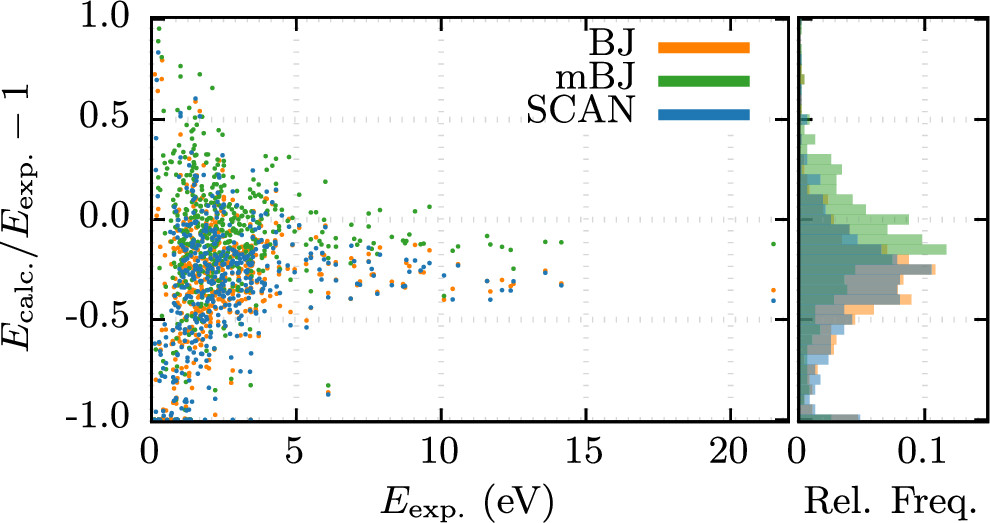
\includegraphics[scale=0.3]{method/dft/metagga.jpeg}
\caption{Calculated to experimental band gap measurements of Becke-Johnsoon, modified Becke-Johnson and SCAN functionals \cite{xc_benchmark}}
\end{figure}

\subsection{Hybrid functionals}

The most precise functional known to DFT belong to the family of \textit{hybrid functionals}. Accordingly this method consist of a hybrid between simpler functionals such as LDA, PBE or even meta-GGA and the exact treatment of exchange energy from Hartree-Fock, for example the global hybrid functional PBE0 \cite{pbe0} described as

\begin{equation}
E_\text{xc} ^\text{PBE0} = (1-\alpha)E_x ^\text{PBE} + \alpha E_x ^{HF} + E_c ^{PBE}, 
\end{equation}
 where alpha is the mixing parameter to decide the balance between the exchange energy, denoted $x$ of Hartree-Fock with PBE, alike the last term represent the correlation energy from the PBE functional. This parameter alpha is determined empirically, thus making hybrid functional a semi-empirical model. Obviously considering the exact exchange in Hartree-Fock is a computationally challenging prospect. Heyd-Scuseria-Ernzerhof managed to lower the cost by the concept of Screened functionals that separate the Coloumb interaction into long-range and short-range interaction by a function $erfc(\mu r)$. These are known as HSE functionals \cite{hse}, the overall best functional for accurate band gaps of solids is by many considered to be HSE06 \cite{hse06} with $\alpha = 0.25$ and $\mu = 0.11$.  
 
\subsection{Outlook} 
 
In many cases LDA and GGA suffice, PBE especially is by most considered the conventional standard for DFT calculations, for its balance of accuracy, cost and wide range applicability. However, distinctly concerning the band gap of a solids, both of these fall short. This is because the band gap of DFT calculations is complicated by the fact that the derivative of the XC-functional is discontinues with respect to the electron concentration \cite{xc_derivative}, thus the simpler functionals fail to recall the experimental values since the total band gap in DFT is the fundamental gap (valence - conduction) + this contribution. This is corrected in meta-GGA and hybrid functionals in the generalized Kohn-Sham scheme. Lastly, we would like to refer the reader to the work of Borlido, Aull, Huran, Tran, Marques, and Botti whom in 2019 conducted an exhastive investigation of the band gap of over 470 uniqe non-magnetic compounds in order to benchmark the relative performance of several of the available and wideley used XC-functionals \cite{xc_benchmark}. In this large-scale project they found overwhelming confirmation that the HSE06 functional followed closely by Modified-Becke Johnson is the superior choice for accurate band-gap measures. Regarding the SCAN functional, in several cases this yielded outputs very comparable to MBJ, and produce much better formation energies than PBE, but tend to overstimate in magnetic alloys. On the other hand the LDA and PBE functional resulted in $50\%$ and $30\%$ under-estimation of the band gap and several cases of miss-classified metals, this was particularly evident in compounds containing Ni and other 3d elements. This result in a limited application to for example narrow gap thermoelectrics or photovoltaics where accurate values of the band gap and states at the band edges is critical.  
 

\section{Fundamental aspects of practical DFT calculations}
\textbf{Needs work, see mainly DFT book ch 3}
With the exchange-correlation functionals presented above, we now have everything in order to perform DFT calculations. To begin solving eq .., we need the single-electron wave-function, for a free electron this is a plane wave $\psi_k = Ae^{i\boldsymbol{k}\boldsymbol{r}}$. In a solid however, there exist a nonzero periodic potential $V(\boldsymbol{r}) = V(\boldsymbol{r} + \boldsymbol{R})$, the solution to the Shr\"{o}dinger equation is given by Bloch's theorem wich states that the solution takes the form
\begin{equation}
\psi_{\boldsymbol{k}}(\boldsymbol{r}) = u_{\boldsymbol{k}}(\boldsymbol{r})e^{i\boldsymbol{k}\boldsymbol{r}},    
\end{equation}
where $u_{\boldsymbol{k}}(\boldsymbol{r})$ is a bloch wave with the periodicity of the supercell, and $\boldsymbol{k}$ is the wavevector. Similar to eq(above), k-space, or reciprocal space is useful to solve the numerous mathematical problems posed by DFT. For instance a great deal of DFT calculations revolve around solving the integral 
\begin{equation}
    g = \frac{V_{\text{cell}}}{(2\pi)^3} \int_{\text{BZ}} g(\boldsymbol{k})d\boldsymbol{k},
\end{equation}
with BZ denoting that the integral be evaluated for all $\boldsymbol{k}$ in the Brillouin zone. This integral can be approximated by evaluating the integral at a set of discrete points and summing over the points with appropriatly assigined weigts. A larger set of points leads to more exact approximations. This method is called Legendre quadrature. The method for selceting these points in reciprocal space was devolped by Monkhorst and Pack in 1976, and simply put requieres a amount of kpoints in each direction in reciprocal space, in the form $N x N x N$. Recalling that reciprocal space is inverse to regular space, supercells with equal and large dimensions converge at smaller values of N, and inversly for cells of small dimsion. In supercells with different length axis, such as hexagonal cells, we use the notation $N x N x M$, where $M$ relate to the distincntly different axis. The amount of kpoints required can be fruther reduced by utulizing the symmetry of the cell, in which we can exactly approximate the entire BZ by extending a lesser zone through symmertry. This reduced zone is appropriartly named the irreducible Brillouin zone (IBZ). 

Metals in particular requiere a large set of kpoints to acchive accurate results. This is becouse we encounter discontinuies functions in the Brillouin zone around the fermi sufrace where the states discontinusly change from occupied to non-occupied. To reduce the cost of this operatin, there are two primary methods, tetrhaedon and smearing. The idea behind the tetrahedon method is to use the discrete set of k-points to fill the reciprocal space with tethraeda and interpolate the function within each tethraeda such that the function can be integrated in the entire space rather than at discrete points. The latter approach for solving discontinuos integrals is to smear out the discontinuity and thus transforming the integral to a continous one. A good analogy to this method is the fermi-dirac function, in which a small variable $\sigma$ transform a step-functino into a continious function that can be integrated by standard methods.

In addition to the number of kpoints, there is one more distinct parameter that must be specified in DFT calculations, namely the energy cutoff, or $E_{\text{cut}}$. This parameters arise from the Bloch function described previosly. In which $u_{\boldsymbol{k}}(\boldsymbol{r})$ was a bloch wave with the same periodicity as the supercell. This implies that the wave can be expanded by a set of special plane waves as
\begin{equation}
    u_{\boldsymbol{k}}(\boldsymbol{r}) = \sum_{\boldsymbol{G}} c_{\boldsymbol{G}}e^{i\boldsymbol{G}\boldsymbol{r}},
\end{equation}
where $\boldsymbol{G}$ is the reciprocal lattice vector. Combining this with eq ..(first eq for blcoh function) we get 
\begin{equation}
    \psi_{\boldsymbol{k}}(\boldsymbol{r}) = \sum_{\boldsymbol{G}} c_{\boldsymbol{k} + \boldsymbol{G}}e^{i(\boldsymbol{k} + \boldsymbol{G})\boldsymbol{r}}
\end{equation}
The consequense from this expression is that evaluating the wavefunction of an electron at a single $k$ point demand a summation over the entirity of reciprocal space. In order to reduce this computational burden, we can introduce a maximum paramater $E_{\text{cut}}$ to cap the calculations. This is possible becouse eq ..(above) is the solution of the Shr\"{o}dinger equation with kinetic energy 
\begin{equation}
    E = \frac{\hbar^2}{2m}|\boldsymbol{k} + \boldsymbol{G}|^2.
\end{equation}
Seeing as the solution with lower energies are the most interesting, we can limit the calculations of eq ..(2 above) to solutions with energy less than $E_{\text{cut}}$ given bellow
\begin{equation}
    E_{\text{cut}} = \frac{\hbar^2}{2m}G_{\text{cut}}.
\end{equation}
Thus, we can reduce the infinitly large sum above to a much more feasable calculation in 
\begin{equation}
    \psi_{\boldsymbol{k}}(\boldsymbol{r}) = \sum_{|\boldsymbol{k} + \boldsymbol{G}| < G_{\text{cut}}} c_{\boldsymbol{k} + \boldsymbol{G}}e^{i(\boldsymbol{k} + \boldsymbol{G})\boldsymbol{r}}
\end{equation}

\textbf{A summary on kpoints and ENCUT, plus a discussion on nummerical convergence and how to select kpoints and ENCUT}


A final consideration to how DFT is applied in practise is how the core electrons are handled. Tightly bound core electrons as opposed to valene electrons demand a greater number of plane-waves to converge. The most efficient method of reducing the expenses of core-electrons are so-called pseudopotentials. This method works by approximating the electron density of the core elecrons by a constant density that mimic the properties of true ion core and core electrons. This density is then remained constant for all subsequent calculations, ie only considering the valence electrons while regarding the core electrons as frozen-in. There are currently two popular types of psudopotentials used in DFT, so-called ultrasoft psudopotentials (USPPs) devoplped by Vanderbilt, and the projecter augmented-wave (PAW) method by Bloch \cite{PAW1}, \cite{PAW2}.

\section{Self-consistent field calculation}
\textbf{Needs work, see lecture notes ch 8, book ch1}
Preceding this section, we have considered the fundamental theory of DFT and it's practical ability to model various materials. In figure \ref{sfDFT} we present the self-consistent field calculation scheme for how DFT calculations are performed. The initial problem posed by dft is that all properties rely on the density, and are dependent on each other. For instance, the effective potential is dependent on the density, which again is dependent on the eigenfunctions, that rely on the effective potential again. The cleaver approach, as seen in figure \ref{sfDFT} begin with an initial guess to the density from which we can solve the Kohn-Sham equation and obtain the corresponding eigenfunctions. Following is an iterative method where we apply the recently calculated eigenfunctions to determine a new density and repeat the procedure above. This is repeated until the total energy is converged, by an own-defined criterion. Equivalently, the optimal ionic positions can be found by a similar approach. This method is based on quasi-Newton algorithms to minimize the forces between ions. 

\begin{figure}
\centering
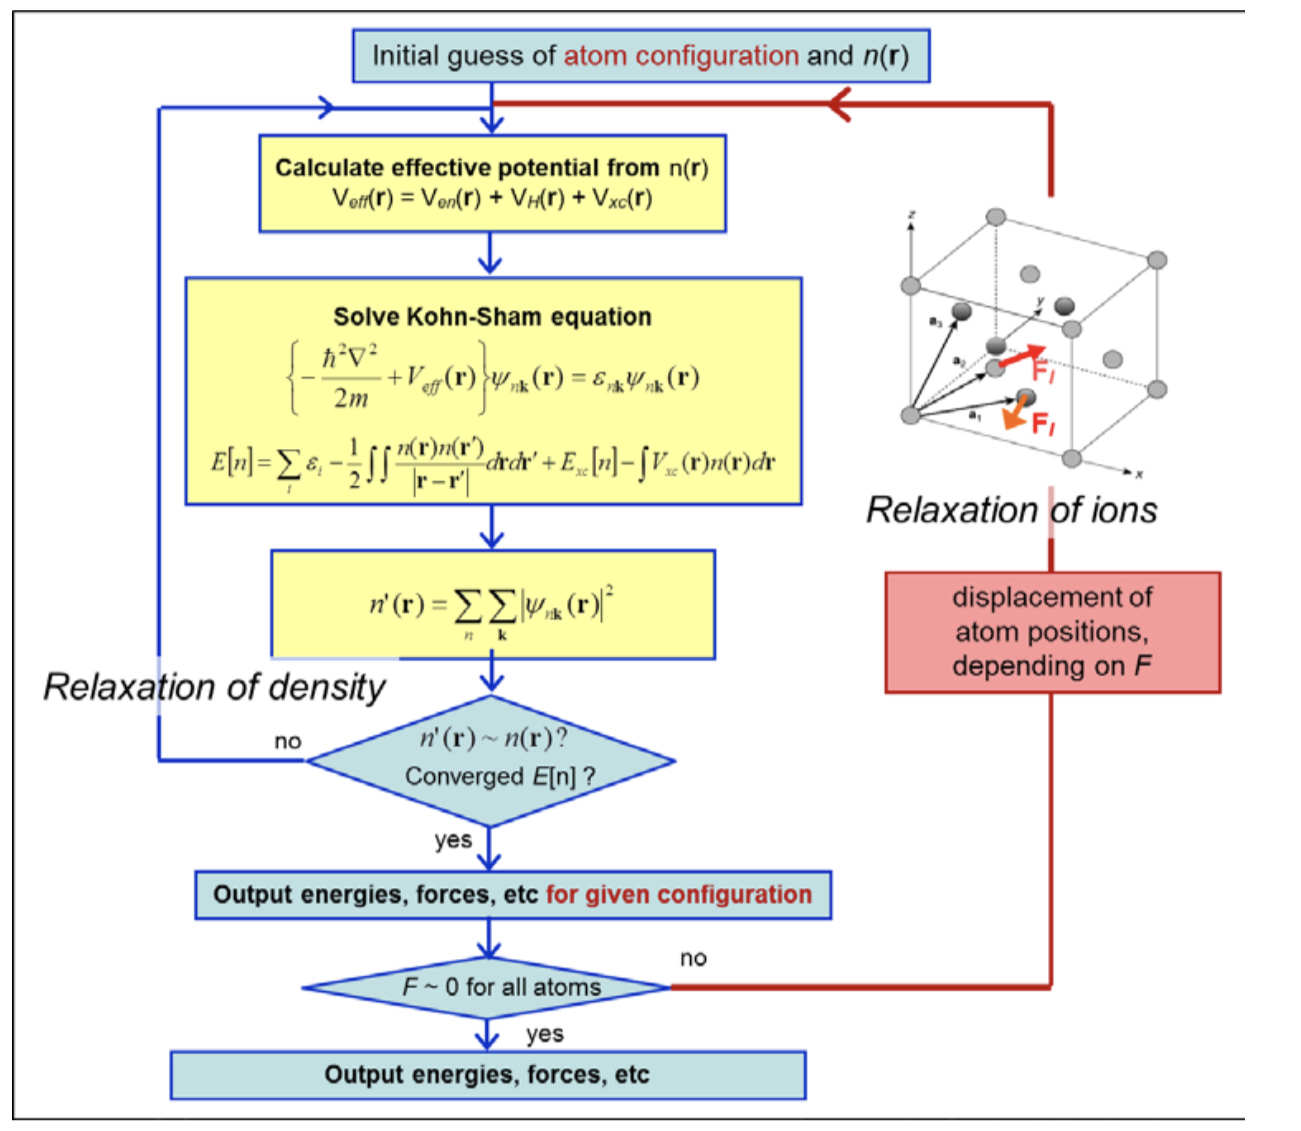
\includegraphics[scale=.3]{theory/selfConsistentDFT.jpeg}
\caption{Self consistent iteration of a DFT calculation. Figure adopted from lecture notes fys-mena4111 \textbf{cite}}
\label{sfDFT}
\end{figure}

